\chapter{Building Blocks of WSN} \label{Chp: Building Blocks}

%In this chapter, we will start by introducing the building components of WSN, mainly focuses on different protocol options at each layer. Then we move to security related work, in three aspects of traffic analysis attacks against different Internet applications, attacks against certain protocols and methods for detecting information leakage in different scenarios. Finally we conclude the chapter by cross referencing those  attacks on Internet to the observable metadata in WSN, proposing the potential traffic features that may lead to information leakage.
In this chapter, we introduce the building blocks of a WSN by OSI model\cite{OSI}.

In OSI model, the data channel is constructed layer by layer from the physical medium at the bottom to the abstracted application at the top (\Cref{fig: OSI model}). Each layer serves a specific purpose, from how to transmit a bit between two physically connected devices to how applications interprets the data. by introducing different protocol options at each layer.

Before the application data is being sent over the wire, two ends of the communication must agree on protocols being used at each layer. The data is then encapsulated from top layer down to the bottom, as depicted in \Cref{fig: OSI channel}. Each encapsulation adds additional metadata, namely protocol headers, to the data. The process is unwound at the receiving side. Normally lower layer protocols are transparent to upper layers.The outputted encapsulated data from upper layer is simply treated as the payload to a lower layer protocol.

In many cases the boundaries between top three layers are ambiguous; thus they are all referred as Application Layer for convenience.
\begin{figure*}
	\centering
	{
		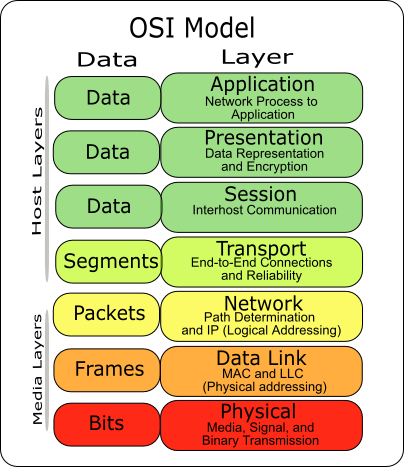
\includegraphics[width=0.4\textwidth,]{fig/Osi-model-jb.png}
	}
	\caption{OSI model} \label{fig: OSI model}
\end{figure*}

\begin{figure*}
	\centering
	{
		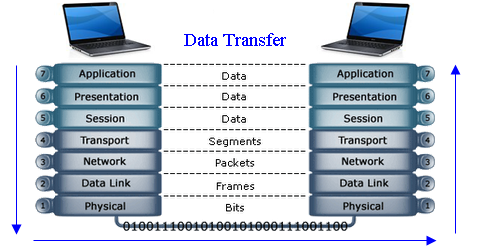
\includegraphics[width=0.6\textwidth,]{fig/osi-model.png}
	}
	\caption{Data Transfer in OSI model} \label{fig: OSI channel}
\end{figure*}

In network terminology, 8 bits is called an OCTET. For the purpose of readability we use the general computer science term BYTE to represent the unit consists of 8 bits.

A combination of protocols at each layer is called a protocol stack, or a protocol suite. The protocol stack until application layer are usually handled by the operating systems. There are several systems specifically aimed to support WSN applications. Contiki\cite{Contiki} is a highly customisable system with 6LoWPAN protocol stack with many hardware supported, OpenWSN\cite{OpenWSN} also has a well hardware support and is featuring full protocol support up to CoAP\cite{rfc7252}, FreeRTOS\cite{FreeRTOS} is optimised for real time tasks, etc.

Due to popularity, in this report we mainly focus on Contiki and the 6LoWPAN protocol stack.

\section{Physical Layer}
Physical Layer specifies the hardware requirements for devices. It defines data transmission at bit level.

WSN features, as explained by its name, wireless connectivity. 802.15.4\cite{802154} standard is supported in many recent WSN devices. Its Physical Layer specification is intended to be for embedded devices emphasising low energy, low cost and low speed. Bluetooth Low Energy, BLE, is another candidate for WSN with similar features. \cite{802154BLE} provides a performance analysis of 802.15.4 and BLE.

Usually the length MAC frame, which we explain in \Cref{Sec: Data Link Layer}, is announced before it is being transmitted, e.g. shown in \Cref{Fig: 802.15.4 PHY Frame}.

\begin{table}[h!]
	\centering
	\begin{tabular}{|l|l|l|l|}
		\hline
		Preamble & SFD & MAC frame Length & Reserved \\ \hline
	\end{tabular}
	\caption{802.15.4 PHY Frame}
	\label{Fig: 802.15.4 PHY Frame}
\end{table}

Preamble is used for hardware synchronisation. Start Frame Delimiter is a constantly 0xE5 for 802.15.4 frames. The length of a MAC frame is 0 to 127 bytes. More details can be found in \cite{802154}.

\section{Data Link Layer} \label{Sec: Data Link Layer}
Data Link Layer solves the problem of how the media is controlled. It also defines the atomic data chunk, called frames, being transmitted over the physical channel. Data Link protocols are strongly related to physical features of underlining devices. This layer is sometimes referred as MAC layer and the frame is called MAC frame in many context. MAC protocol only solves single hop communication. Packet forward is defined in upper layer protocols.

With respect to Media Access Control, MAC, technologies such as CSMA/CA \cite{802154} standard and TSCH\cite{TSCH} provides solutions to at which timing and channel should the radio transceiver send and receive data. ContikiMAC\cite{ContikiMAC} proposes a Radio Duty Cycle, RDC, protocol that aims to be energy efficient and has been implemented on Contiki OS.

Another major component in Data Link Layer protocols is the format of different types of frames. In this research, we focus on 802.15.4 standard as its increasing attention in both industry and academy. 

Implementing security measures at this layer is called Link Layer SECurity, LLSEC. 

\subsection{802.15.4 MAC Layer} \label{Subsec: 802.15.4 MAC Layer}

There are four types of frames defined in this standard, which are:
\begin{description}
	\item[\textbf{Beacon}] broadcastes to physically organise the network.
	\item[\textbf{Command}] is used in network maintenance.
	\item[\textbf{Data}] carries actual payload.
	\item[\textbf{ACK}] only optionally sent in response when requested.
\end{description}

Among these types of frames, we are particularly interested in Data frames. We will explain our concern of this choice later in \Cref{Sec: Leakage Sources}. \Cref{Fig: 802154 frame} describes the format of a 802.15.4 Data frame.

\begin{figure*}[h!]
	\centering
	\begin{tabular}{|c|c|c|c|c|}
		\multicolumn{3}{c}{\textit{MAC Header}}                           & \multicolumn{1}{c}{\textit{MAC Payload}} & \multicolumn{1}{c}{\textit{MAC Footer}}     \\ \hline
		2 (bytes)     & 1                    & 4 to 20              & *           & 2              \\ \hline
		Frame Control & Data Sequence Number & Address Information & Data        & Frame Checksum \\ \hline
	\end{tabular}
	\caption{802.15.4 Data Frame}
	\label{Fig: 802154 frame}
\end{figure*}

We briefly explain the format of 802.15.4 Data frame.
\begin{description}[style=nextline]
	\item[\textbf{Frame Control}]
	This 2 bytes field contains the bit flags of additional information that instructs how the receiver should interpret this frame, including the type of this frame, whether the security option is enabled and how the source and destination addresses are represented. When the security option is enabled, additional field will be added to the frame. We will explain the security enabled frame format later in \Cref{Sec: Data Link Layer}. A full explanation of the flags can be found in \cite{802154}.
	
	\item[\textbf{Sequence Number}]
	Each packet is assigned a sequence number. The main purpose of this field is that it enables a simple acknowledgement mechanism, ACK, at MAC layer. Since MAC layer provides only unreliable transmission, i.e. MAC frames are allowed to be dropped or arrive disordered; hence the ACK is optional. However, some other protocol can utilise this ACK, e.g. ContikiMAC uses the ACK MAC frame to inform the sender that the frame is received and hence terminates the resending process of sender.
	
	\item[\textbf{Address Information}]
	This field contains the source address and destination address of this frame. The length of address is variable. Simply speaking, a longer addresses is used for larger network. and shorter for smaller. Each device has a unique built in address as known as MAC address. The MAC address is configurable on some, in fact nearly all recently, devices. Broadcast is achieved by using a specific destination address but group multicast is not implemented on this layer. In fact, given the physical character of radio, both broadcast messages and unicast messages are technically broadcasted. It entirely depends on the receiver to dropping frames that specifies an unicast address of other nodes.
	
	\item[\textbf{Data}]
	This is the MAC layer data. This data is constituted of upper layer protocol headers and application data.
	
	\item[\textbf{Frame Checksum}]
	The checksum is used to check and correct the error induced by physical channel.
\end{description}

The Frame Control, Sequence Number and Address Information together are called MAC header. The Data field is called MAC payload accordingly. 

802.15.4 standard specifies the Maximum Transmission Unit, MTU, to be 127 bytes including the MAC header and footer. That is to say any 802.15.4 compatible hardware must be able to send at least 127 bytes within one frame; any frame that is larger than this size is not guaranteed to be support by the device. Since the MAC header and footer consumes 25 bytes in a Data frame, there is actually 102 bytes left for MAC payload.

Setting the security flag in Frame Control enables 802.15.4 security and adds additional information into the MAC header. We introduce the 802.15.4 security later in \Cref{Subsec: 802154 Sec}.

\subsection{802.15.4 Security} \label{Subsec: 802154 Sec}
802.15.4 security is based on symmetric cryptography, namely Authenticated Encryption with Associated Data, AEAD, scheme. To be more specifically, it provides encryption for MAC payload and authenticity for both MAC header and payload. The cryptographic primitive adopts AES-128 as the block cipher.

802.15.4 has a set of configurable security levels:
\begin{itemize}
\item Encryption only, i.e. only MAC payload is encrypted in CTR mode.
\item Authentication only, i.e. a tag is attached at the end of Data field. The tag is computed on MAC header and MAC payload in CBC mode. The MAC payload is transmitted in plaintext.
\item Encryption and authentication. The whole frame is processed in CCM*\cite{802154} mode, with MAC header being the associated data and MAC payload being the plaintext to be encrypted. The asterisk symbol represents a slight restriction which requires the nonce, or IV, must contain the encoded format specifier that can uniquely determine the format of output ciphertext. In other words, the receiver must can uniquely determine solely by nonce whether authentication and encryption are enabled as well as the length of authentication tag.
\item The tag can be further configured to be 32 bit, 64 bit or 128 bit when authentication is enabled.
\end{itemize}

The format of a 802.15.4 Data frame with security option set is described in \Cref{Fig: 802154 sec frame}.

\begin{figure*}[h!]
	\centering
	\begin{tabular}{|c|c|c|c|c|c|c|}
		\multicolumn{4}{c}{\textit{MAC Header}}                                                             & \multicolumn{2}{c}{\textit{MAC Payload}} & \multicolumn{1}{c}{\textit{MAC Footer}}     \\ \hline
		\multicolumn{3}{|c|}{\multirow{2}{*}{As MAC header in \Cref{Fig: 802154 frame}}} & 0 to 14                    & *             & 0/4/8/16         & 2              \\ \cline{4-7} 
		\multicolumn{3}{|c|}{}                                           & Auxiliary Security Header & Data          & MIC              & Frame Checksum \\ \hline
	\end{tabular}
	\caption{802.15.4 Frame with security option enabled} \label{Fig: 802154 sec frame}
\end{figure*}

The Auxiliary Security Header contains the additional information needed by 802.15.4 security.

\begin{description}[style=nextline]
	\item[\textbf{Security Level}]
	Security Level is represented by the first 3 bits in Auxiliary Security Header. The highest bit controls whether encryption is enabled. The lower two bits controls the length of MIC with the value $0$ indicates no authentication.
	\item[\textbf{Frame Counter}]
	This 4 byte filed increases by one for each frame sent. It is also used for replay detection.
	\item[\textbf{Key Strategy}]
	The other parts instructs which key to be used for this frame. The keys are presumed to be pre-shared in PAN Information Base, PIB, which is a database containing information that is shared among the network. Keys are managed by groups and indexes within a group. The definition of groups depends on upper layer applications.
\end{description}

More details of Auxiliary Security Header is defined in the 802.15.4 standard.

Message Integrity Code, MIC, is equivalent to the cryptography term Message Authenticate Code, MAC. Therefore the term MIC is used to avoid confusion with Media Access Control.

Access Control List, ACL, is a list data structure defined in 802.15.4. It is used to maintain 802.15.4 security access during runtime.Each entry in ACL is paired with another node.  An ACL entry contains the following elements:
\begin{description}
	\item[\textbf{Address}] The address of remote node, used as an identifier.
	\item[\textbf{Security Suite}] The security level to use associated to the address.
	\item[\textbf{Key}] The paired cryptographic key associated to the address.
	\item[\textbf{Last Initial Vector}] Nonce used for the last outgoing frame.
	\item[\textbf{Replay Counter}] Nonce received for the last incoming frame.
\end{description}
On sending a frame with security option, the sender looks up destination address in ACL and determines the security level, key and frame counter which is encoded into the last initial vector. On receiving a frame, the receiver looks up source address in ACL and checks for match of the security suite and security level in the frame. Then it verifies the frame with the key. If replay protection is enabled, the replay counter is also compared. Failing any of the tests will result into rejecting of the frame.

\subsection{Nonce of CCM* in 802.15.4 security}
As stated earlier in \Cref{Subsec: 802154 Sec}, CCM* requires that the format of ciphertext can be uniquely deduced from the nonce. \Cref{Fig: CCM nonce} describes the nonce used for encryption.

\begin{figure*}[h!]
	\centering
	\begin{tabular}{|c|c|c|c|c|}
		\hline 
		1 (bytes) & 8              & 4             & 1              & 2             \\ \hline
		Flag      & Source Address & Frame Counter & Security Level & Block Counter \\ \hline
	\end{tabular}
	\caption{CCM* nonce for encryption}
	\label{Fig: CCM nonce}
\end{figure*}

\begin{description}
\item[\textbf{Flag}]
This is a constant a value equals to 0x02.
\item[\textbf{Source Address}]
This field is the address of sender. If an address of length than 8 byte is used, it will be extended to 8 byte.
\item[\textbf{Frame Counter}]
The frame counter is directly mapped from the same filed in Auxiliary Security Header, as described earlier.
\item[\textbf{Security Level}]
As of frame counter, security level is also directly mapped from Auxiliary Security Header with the highest bit set to $0$. As described earlier, security level solely determines the format of ciphertext.
\item[\textbf{Block Counter}]
This is exactly the block index of MAC payload, increases by one for each block. Since AES-128 is the underlining block cipher; therefore the block size is 128 bit.
\end{description}

802.15.4 security could either be implemented by hardware and/or software. Some platform may not support the security option, or only supports a sub set of this measure. We briefly describe an implementation on Contiki platform later in \Cref{Subsec: noncoresec}.

\subsubsection{Implementation on Contiki: noncoresec} \label{Subsec: noncoresec}
noncoresec is the LLSEC implementation on Contiki. It is a reduced implementation of 802.15.4 security which supports only a network shared key hard coded into the kernel code.

\subsection{Sub Layer: RDC Layer}
In practical, the radio transceiver turned out to be the most energy consuming part in a sensor node. Further more, listening data consumes more energy than sending them. Thus an optimisation for energy preserving is to switch off the transceiver for most of the time and switch it on only when there is data on air. The Radio Duty Cycle, RDC, Sub Layer is therefore added to MAC Layer. RDC protocols control the behaviour of radio transceiver by synchronise their timing of sending and receiving data; hence the radio can be kept off for most of the time. In the case of Contiki, there are two RDC protocols implemented:
\begin{itemize}
\item \textbf{nullrdc}. There is no RDC protocol. The transceiver is kept on forever.
\item \textbf{ContikiMAC\cite{ContikiMAC}}. The transceiver is kept off for most of the time and only wakes up for a short period. If data transmission is detected during the wake-up period, the receiver keeps the transceiver on until the frame is received and informs the sender with an ACK. On the other hand, the sender continuously retransmits the frame until an ACK is received or the time runs out.
\end{itemize}

Time-Slotted Channel Hopping\cite{TSCH}, TSCH, is another RDC protocol that is adopted by OpenWSN. Since it is not implemented yet in our platform, Contiki, we omit its further details in this report.

\section{Network Layer}
The Data Link Layer protocol has solved the problem of data transmission over directly linked nodes. However, real world WSN applications are sometimes deployed in a wider range that not all nodes can be directly connected, such as a smart city application. The solution to build a logic data path between the nodes where each intermediate node forwards the data to the next node until it reaches its destination. Such logical data path is called a multi hop connection and directly connected data path is called a single hop connection respectively. The transmission unit at the Network Layer is called a packet.

A network is defined as a set of nodes logically connected to each other. There are two common types of network considered in WSN applications:
\begin{description}[style=nextline]
	\item[\textbf{Star Network}]
	Star network is a centralised network, as in \Cref{fig: Star Network}. Each node is directly linked to the centre. Star networks can be easily implemented and thus requires less resources.
	\item[\textbf{Mesh Network}]
	Mesh network has a decentralised structure as shown in \Cref{fig: Mesh Network}. Every node is capable to forward packets. Comparing to star network, mesh network is more flexible and scalable but also more complicate and harder to implement. Mesh network is more practical than star network in large scale applications, such as smart cities.
\end{description}

\begin{figure*}
	\centering
	\begin{subfigure}[b]{0.5\textwidth}
		{
			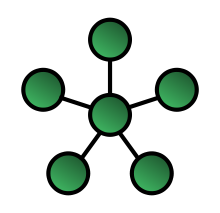
\includegraphics[width=0.5\textwidth,]{fig/StarNetwork.png}
		}
		\subcaption{Star Network} \label{fig: Star Network}
	\end{subfigure}
	\begin{subfigure}[b]{0.5\textwidth}
		{
			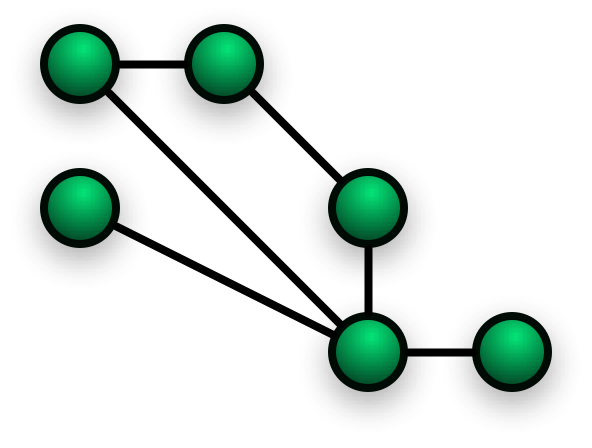
\includegraphics[width=0.5\textwidth,]{fig/NetworkTopology-Mesh.png}
		}
		\subcaption{Mesh Network} \label{fig: Mesh Network}
	\end{subfigure}
	\caption{Network Topologies} \label{fig: Network topologies}
\end{figure*}

Some network are built with a hybrid approach of star network and mesh network, e.g. the Cluster Tree Network of Zigbee\cite{Zigbee} as showed in \Cref{fig: ZigBee Topologies}.

\begin{figure*}[h!]
	\centering
	{
		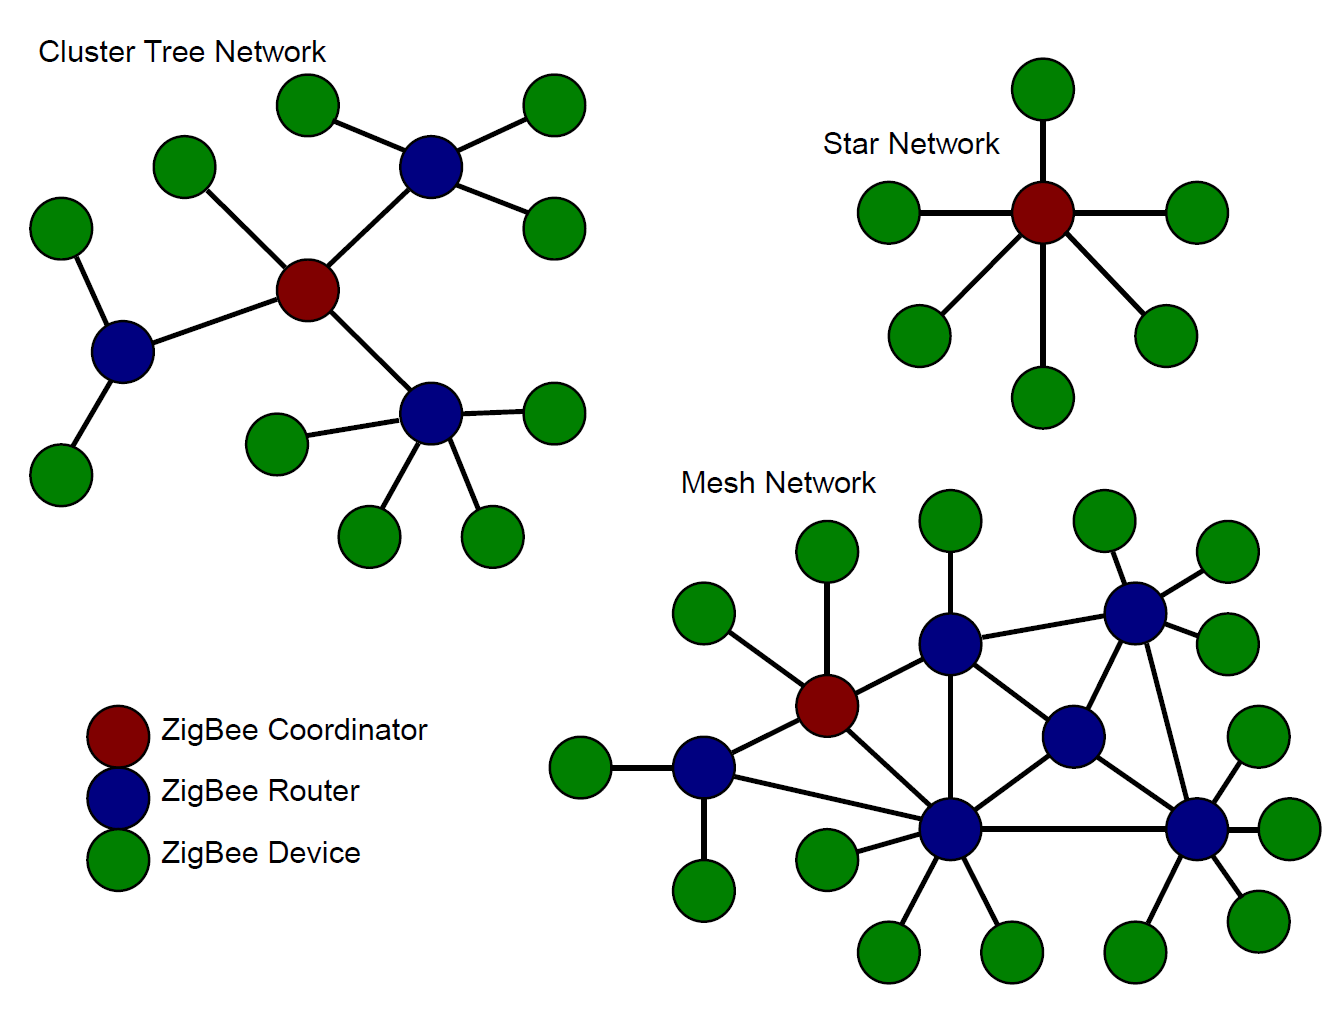
\includegraphics[width=0.7\textwidth,]{fig/ZigBeeTopologies.png}
	}
	\caption{Different ZigBee Network Topologies} \label{fig: ZigBee Topologies}
\end{figure*}

6LoWPAN is a currently well adopted network standard. It has the following features making it popular in IoT industry: 
\begin{itemize}
	\item Each device is assigned with an IPv6 address of compressed format. With a border router that translates the compressed IPv6 address into an IP address, a node inside 6LoWPAN  can directly communicate with a host over Internet.
	\item Its mesh routing feature lead to a flexible, scalable and robust network, as the network can spontaneously reorganise itself at running time.
	\item It is standardised by IETF and well supported in industry.
\end{itemize}

As of this project, we are particularly interested into 6LoWPAN due to the reasons above. Packets in a 6LoWPAN can be categorised into two classes:
\begin{enumerate}
	\item \textbf{IPv6 Data Packets}
	\item \textbf{ICMPv6 Packets}
\end{enumerate}
We give a brief explanation of their contents in \Cref{Subsec: IPv6 Data Packets} and \Cref{Subsec: ICMPv6} respectively.

\subsection{6LoWPAN Adaptation Sub Layer} \label{Subsec:6LoWPAN Adaptation Sub Layer}
A sub layer is defined in 6LoWPAN standard\cite{rfc4944} to compress a standard IPv6 header, in order to reduce the overhead induced by protocol stacks and provide more bandwidth to the applications. Additional headers are prepended before the IPv6 header as shown in \Cref{Fig: 6LoWPAN Adaptation Header}. 

\begin{figure*}[h!]
	\centering
	\begin{tabular}{|l|l|l|}
		\hline
		6LoWPAN Adaptation Header & Compressed IPv6 Header & IPv6 Payload \\ \hline
	\end{tabular}
	\caption{6LoWPAN Adaptation Header}
\label{Fig: 6LoWPAN Adaptation Header}
\end{figure*}

The header compression is generally done by:
\begin{itemize}
	\item Optimised encoding. Take the Hop Limit, HLIM or TTL (Time To Live), field for example, the frequently used values, 1, 64 and 255, are represented in 2 bits as 01b, 10b and 11b respectively, saving 6 bits from its original 1 byte field.
	\item Since 6LoWPAN has usually less devices than a normal IPv6 network. The unused higher bits are therefore re-encoded. Technically speaking this is also a kind of optimised encoding.
\end{itemize}
The header compression is a lossless; thus we can always reconstruct an equivalent IPv6 header from the compressed header and this header compression information. We omitted further complicated details due to its complexity but they are defined in \cite{rfc6282}.

In addition to header compression, 6LoWPAN Adaptation Header also contains information for packet fragmentation as well as device address conflict avoiding. We omit the further details as it is beyond the scope of this report. Details of these mechanisms are defined in \cite{rfc4944}.

\subsection{IPv6 Data Packets} \label{Subsec: IPv6 Data Packets}
These packets contains the IPv6 payload. In 6LoWPAN, the IPv6 header is compressed as described in \Cref{Subsec:6LoWPAN Adaptation Sub Layer}. In this section we explain the contents of a standard IPv6 header instead of a compressed one for convenience but one can always uniquely transform a standard IPv6 header to a compressed one since they are indeed equivalent.

IPv6 is defined in \cite{rfc2460}. Its basic format is as shown in \Cref{Fig: IPv6 Packet Format}. We removed the length information as they are inconsistent when the header is compressed.

\begin{figure*}[h!]
\center
	\begin{tabular}{l|c|c|c|c|c|c|}
	\cline{2-7}
	\multirow{2}{*}{\textit{IP Header}} & Version & Traffic Class & Flow Label & Payload Length & Next Header & Hop Limit \\ \cline{2-7} 
	                                & \multicolumn{3}{c|}{Source Address}  & \multicolumn{3}{c|}{Destination Address} \\ \cline{2-7} 
	\textit{IP Payload}                 & \multicolumn{6}{c|}{Payload}                                                    \\ \cline{2-7} 
	\end{tabular}
	\caption{Basic IPv6 Packet Format} \label{Fig: IPv6 Packet Format}
\end{figure*}

\begin{description}[style=nextline]
	\item[\textbf{Version}]
	In 6LoWPAN this is constant 0x6.
	\item[\textbf{Traffic Class}]
	This field is default by 0 and may be set by an upper layer application as a hint of packet. A router can act accordingly to this field, such as adjusting the priority of packet, or even modify this value upon forward. The support for values other than $0$ is optional.
	\item[\textbf{Flow Label}]
	This field is intended to label a logical data path at Network Layer. The IPv6 standard\cite{rfc2460} states  it should ``be used by a source to label sequences of packets for which it requests special handling by the IPv6 routers, such as non-default quality of service or `real-time` service``. Support to this field is optional.
	\item[\textbf{Payload Length}]
	This field specifies the length of Network Layer payload.
	\item[\textbf{Next Header}]
	This field specifies the Transportation Layer protocol to be used. In WSN applications this is usually UDP. We will cover more of this in \Cref{Sec: Transportation Layer}.
	\item[\textbf{Hop Limit}]
	Hop Limit, HLIM, is also called Time To Live, TTL. It decreases by one whenever the packet is forwarded. The packet will be dropped when this value reaches $0$. This prevents a packet from being infinitely forwarded.
	\item[\textbf{Source Address and Destination Address}]
	These are the IPv6 addresses of sender and receiver. These are addresses are normally consistent during routing of a packet. In comparison,MAC source and destination varies on each hop, as an intermediate receiver becomes the sender of next hop.
	\item[\textbf{Payload}]
	This field contains the upper layer protocol headers and application data.
\end{description}
One thing to be noticed is that Traffic Class and Flow Label is not yet fully defined by IPv6 standard.

There are also extension headers defined in IPv6\cite{rfc2460}, including IPsec and fragmentation ,etc.

IPsec is defined in \cite{rfc4301} with its Authentication Header, AH, defined by \cite{rfc4302} and Encapsulating Security Payload, ESP, defined by \cite{rfc4303}. AH authenticates all IP Headers (the basic IPv6 header and the extensions) except fields  those might be modified by a router such as TTL. ESP provides encryption over IP Payload. Enabling IPsec over IPv6 adds 40 bytes to the IP Header which is unacceptable in IoT environment. \cite{6LoWPANIPsec} and \cite{CompressIPsec} discusses compression of IPsec over 6LoWPAN. \cite{ContikiIPsec} describes an implementation of IPsec over Contiki but it is not yet adopted by the latest released Contiki 3.0.

We omit further details of other extension headers as they are mostly used to handle routing and fragmentation and thus beyond the scope of this report.

\subsection{ICMPv6 Packets} \label{Subsec: ICMPv6}
Internet Control Message Protocol for IPv6, ICMPv6, is a set of messages that are used to maintain the network. \cite{rfc4443} defines the general format alongside with ICMPv6 Error Messages and Information Messages. 

%IPv6 General Format
In IPv6, an ICMP messages is preceded by an IPv6 Basic Header and optional IPv6 extension headers with the last Next Header field set to ICMP as \Cref{Fig: ICMP with IPv6}. The IP Payload in \Cref{Fig: IPv6 Packet Format} is replaced by an ICMP message in this case.

\begin{figure*}[h!]
	\centering
	\begin{tabular}{|l|l|l|}
		\hline
		IPv6 Basic Header & Extension Headers (optional) & ICMP Message \\ \hline
	\end{tabular}
	\caption{ICMP Message with IPv6 Headers}
	\label{Fig: ICMP with IPv6}
\end{figure*}

The general format of an IPv6 message is described in \cite{rfc4443} as \Cref{Fig: General Format of ICMPv6 Message}.
\begin{figure*}[h!]
	\centering
	\begin{tabular}{|c|c|c|c|}
	\hline
	1 (byte) & 1    & 2        & *            \\ \hline
	Type     & Code & Checksum & Message Body \\ \hline
	\end{tabular}
	\caption{General Format of ICMPv6 Message}
	\label{Fig: General Format of ICMPv6 Message}
\end{figure*}

As stated in \cite{rfc4443},
\begin{description}[style=nextline]
\item[\textbf{Type}]
There are two groups of types of messages defined in \cite{rfc4443}. Error messages have a Type value in $[0,127]$ which indicates an error of network. Information messages have a type value in $[128,255]$ which provide network information to nodes of the network.
\item[\textbf{Code}]
Each type of ICMP message defines its own code to indicate the exact functionality of an ICMP message.
\item[\textbf{Checksum}]
Checksum for the packet.
\end{description}

We explain only a minor set of ICMP Messages that we have successfully observed in our experiment.
%Error messages, informative message
\begin{description}[style=nextline]
\item[\textbf{Echo Request and Reply Messages}]
These are diagnostic ICMP Information messages. Upon receiving an ICMP Echo Request, the receiving node is required by \cite{rfc4443} to reply with an identical ICMP message except the source and destination addresses are inverted. The Echo Request is typically sent by a PING command for diagnostic reasons such as testing of connectivity or measuring the Round Trip Time, RTT, of a data path. The response of ICMP Echo is enabled in Contiki by default but it is disabled on many Internet server for security reasons.
\end{description}

%RPL messages
A family of ICMPv6 messages, RPL messages, are defined by \cite{rfc6550}. RPL messages are fundamental in forming and self-organising a 6LoWPAN network. A 6LoWPAN network instance is a Destination Oriented Directed Acyclic Graph, DODAG, shown in \Cref{Fig: DODAG}. 
\begin{figure*}[h!]
	\center
	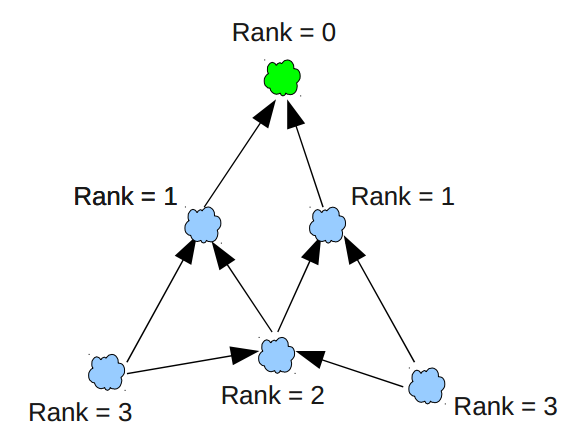
\includegraphics[width=0.6\textwidth]{fig/dodag.png}
	\caption{A DODAG}
	\label{Fig: DODAG}
\end{figure*}
We omit further details of the decision of a routing path as it is beyond the scope of this report but they are defined in \cite{rfc6550}. Instead, we explain the major related ICMP messages in a 6LoWPAN network.
%DODAG Information Solicitation
%DODAG Information Object
%Destination Advertisement Object
\begin{description}[style=nextline]
\item[\textbf{DAG Information Object (DIO) Message}]
The DIO message contains the global information of a 6LoWPAN network. It is broadcasted by a node to its neighbours periodically for maintenance, or as a reply on request of a new joining node to provide enough information for the new one to join the network.

\item[\textbf{DAG Information Solicitation (DIS) Message}]
When a new node is booted, it broadcasts DIS messages probing an existing 6LoWPAN network. If the DIS message is received by any neighbour node that belong to a network, then a DIO message is replied providing the information to join the network.

\item[\textbf{Destination Advertisement Object (DAO) Message}]
DAO Message is sent by a child node to its precedents to propagate its routing information. The routing information is later used when another node tries to send a packet to this child node. The receiving parent can either store the routing information or forward it to an upper level parent depending on its capability.
\end{description}

\cite{rfc6550} also defined secure variants to these RPL messages which provides authentication as well as confidentiality. However, they are not implemented on our platform and therefore we omit their details in this report.

\section{Transport Layer} \label{Sec: Transportation Layer}
Transport Layer defines the interface to applications. To be more specifically, ports are defined at this layer in addition to network addresses allowing packets to be directed to different applications running on the same host. Transport Layer protocols also define more semantic details of the data channel, such as reliability and modes data operation.

TCP and UDP are the most widely used Transport Layer protocols over Internet. TCP provides a reliable streamed data channel whilst UDP provides only unreliable datagrams. In the world of IoT, UDP is generally preferable due to its low overhead and support to multicast.

UDP is defined in \cite{rfc768}. Its format is shown in \Cref{Fig: UDP Datagram Format}
\begin{figure*}[h!]
	\center
	\begin{tabular}{|c|c|c|c|c|}
		\hline
		2 (bytes)   & 2                & 2              & 2        & *       \\ \hline
		Source Port & Destination Port & Payload Length & Checksum & Payload \\ \hline
	\end{tabular}
	\caption{UDP Datagram Format}
	\label{Fig: UDP Datagram Format}
\end{figure*}

\begin{description}[style=nextline]
	\item[\textbf{Source and Destination Port}]
	Ports are the identifier of applications running on a host. The source port and destination port semantically represent the applications that send and receive the data respectively.
	\item[\textbf{Payload Length}]
	The length of UDP payload.
	\item[\textbf{Checksum}]
	Checksum of the packet. The checksum is optional in \cite{rfc768} but is required in 6LoWPAN.
	\item[\textbf{Payload}]
	The application data.
\end{description}

The UDP header constitutes of 8 bytes and contains only the minimum information for the OS to identify the receiving process of a packet. Data transmission of UDP is unreliable, which means the data might be lost or arrive disordered.

The combination of a network address and a port is called an entity in network term.

\section{Application Layer}
%DTLS
%MQTT
%CoAP
This layer represents the various applications on the architecture. Some Application Layer protocols may beneath other applications, such as TLS and DTLS are sometimes viewed as a sub layer protocol of Transport Layer.

In this section we describe two typical Application Layer protocols that has been implemented on our platform, namely DTLS\cite{rfc6347} and CoAP\cite{rfc7252}. A real application can be built on these protocols.

\subsection{DTLS}
DTLS\cite{rfc6347} stands for Datagram Transport Layer Security. As of TLS, it provides end-to-end data confidentiality and authenticity. The main difference between DTLS and TLS is that:
\begin{itemize}
	\item DTLS is built on datagrams instead of TCP like TLS. In case of a 6LoWPAN network, this is effectively UDP. As a result DTLS implemented a simple reliable transmission mechanism during handshake to reliably exchange the cryptographic materials.
	\item Explicit sequence number and epoch values on each DTLS record. We explain theses values in following context.
	\item Invalid records no longer terminate the connection. Instead, errors are suppressed to the upper layer application and an alert is sent.
	\item RC4 is disabled due to its stateful design\cite{DtlsCiphers}. It is hard to maintain synchronised stated with UDP.
\end{itemize}

A packet containing Application Layer data is called a record. The format of a DTLS record is as depicted in \Cref{Fig: DTLS Record Format}.
\begin{figure*}[h!]
	\begin{tabular}{|c|c|c|c|c|c|}
		\hline
		1 (byte)     & 2                & 2     & 6               & 2      & *        \\ \hline
		Content Type & Protocol Version & Epoch & Sequence Number & Length & Fragment \\ \hline
	\end{tabular}
	\caption{DTLS Record Format}
	\label{Fig: DTLS Record Format}
\end{figure*}

\begin{description}[style=nextline]
	\item[\textbf{Content Type}]
	Content Type is inherited from TLS. It indicates the type of this record. The value can either be:
	\begin{enumerate}
		\item CHANGE\_CIPHER\_SPEC($20$)
		\item ALERT($21$)
		\item HANDSHAKE($22$)
		\item APPLICATION\_DATA($23$)
	\end{enumerate}
	In the case of CHANGE\_CIPHER\_SPEC and HANDSHAKE, the sub protocol are invoked accordingly. Otherwise the Fragment field is treated as an error code in case of ALERT or ciphertext of application data in case of APPLICATION\_DATA.
	\item[\textbf{Protocol Version}]
	DTLS uses the complement of \{0xff, 0xff\} to indicate the version number. Since the implementation on our platform is for DTLS 1.2, this field is constantly \{0xfe, 0xfd\}.
	\item[\textbf{Epoch}]
	This field is incremented by one for each cipher state change, such as an invocation of \\
	CHANGE\_CIPHER\_SPEC. This value is used as an index of which set of cryptographic materials to be used, such as algorithms, keys or nonces.
	\item[\textbf{Sequence Number}]
	This field is the sequence number of this record. The sequence number is used by some cryptographic algorithms, such as to form a part of nonce.
	\item[\textbf{Length}]
	The length of Fragment field.
	\item[\textbf{Fragment}]
	The content of Fragment depends on Content Type. In the case of APPLICATION\_DATA, the Fragment contains the ciphertext.
\end{description}

The DTLS on Contiki is implemented by a third party code, tinydtls-0.8.2\cite{tinydtls}. Its current version supports two ciphersuites, namely:
\begin{itemize}
	\item TLS\_ECDHE\_ECDSA\_WITH\_AES\_128\_CCM\_8\cite{rfc7251}
	\item TLS\_PSK\_WITH\_AES\_128\_CCM\_8\cite{rfc6655}
\end{itemize}
Both ciphersuites adopts the same AEAD scheme, AES\_128 with CCM mode, as their cryptographic primitives. Further details of the AEAD scheme is defined in \cite{rfc5116} and \cite{CCM}.

One thing to be noticed is that DTLS is not compatible with the multicast feature of IPv6 and UDP. The direct reason is the distribution of cryptographic materials poses a great difficulty in IoT applications. \cite{DtlsMulticast1} and \cite{DtlsMulticast2} discuss this topic in further details.

As of this project, we are mostly focused on the APPLICATION\_DATA records rather than the handshake process, as we consider the later to be performed independently from any upper layer application.

\subsection{CoAP}
%CoAP as TCP

%\section{Other protocols and standards}
%Zigbee 

\section{Summary}
%Protocol suite